	%------------------第一章---------------------------
	\newpage
	\section{绪论}
    \subsection{超声波接近传感器的研究背景和意义}
    \subsubsection{超声波接近传感器的发展}
    超声波接近传感器是一种能够实现非接触测距的传感器。随着现代工业和科技的快速发展,超声波接近传感器的应用领域也在不断扩大,已经成为自动控制、机器人、无人驾驶等领域中不可或缺的组成部分。其发展经历了三个阶段:第一代采用固定式超声波传感器,第二代采用微机处理技术和数字滤波技术,第三代采用了新型材料和新技术,如MEMS技术、FPGA技术等,提高了系统的测量精度、稳定性和抗干扰能力。在未来,超声波接近传感器将进一步发展,应用领域将更加广泛,并且在系统的设计、制造和使用方面还有许多问题和挑战需要解决和克服。
    \subsubsection{超声波接近传感器国内外研究现状}
    \paragraph{国内研究现状}
    中国的超声波接近传感器研究在过去几十年里得到了快速发展。目前,国内大量高校和研究机构已经开始从事这方面的研究,如清华大学、中国科学院声学研究所、南京大学、哈尔滨工业大学等。在研究领域方面,主要集中在新材料、新结构的超声波传感器、嵌入式系统设计、信号处理与模式识别等方面。
    
    同时,超声波接近传感器在国内工业应用中得到了广泛应用,主要应用于物体距离测量、机器人导航、车辆防撞系统、矿井安全监测等领域。在冶金、石化、化工、航空、航天等行业中,也得到了广泛的应用,取得了显著的经济效益和社会效益。
    
    值得一提的是,近年来,中国在超声波传感器的应用方面也进行了大量的研究和应用,例如,利用超声波技术实现的脑机接口、水下定位和测量等方面,都取得了重要的进展。总之,中国的超声波接近传感器研究已经逐步走向应用,取得了一些具有国际竞争力的成果,为国内相关领域的技术进步和经济发展做出了积极贡献。
    \paragraph{国外研究现状}
    超声波接近传感器在国外也得到了广泛的应用和研究。美国、日本、德国等发达国家的企业和研究机构在超声波传感技术方面取得了很多创新性成果。美国的Honeywell、日本的松下、德国的西门子等公司都是超声波传感器领域的龙头企业。此外,德国的Fraunhofer公司也是超声波技术研究的领军机构之一,他们致力于超声波传感器的研究和开发,取得了一系列重要进展。
    
    在超声波接近传感器的应用方面,国外的应用场景更加广泛,包括物体检测、精度测量、人体检测、障碍物检测等领域。例如,日本的松下公司在机器人领域应用超声波传感器实现了机器人的自主导航功能;德国的西门子公司在工业自动化领域采用超声波传感器实现了物体的非接触式测量。这些成功的应用案例表明超声波接近传感器在未来的发展中具有广阔的应用前景。
    
    \subsubsection{超声波接近传感器的研究意义}
    在现代工业和自动化控制中,超声波传感器已经成为了一种重要的非接触式测量和检测手段。传统的超声波传感器由于受到环境干扰和传感器本身精度等问题的限制,其应用场景和测量范围受到一定的限制。因此,需要一种高精度、低功耗、多功能的超声波传感器来满足实际应用需求。\par
    TUSS4470芯片作为一种新型的超声波传感器芯片,具有高精度、低功耗和多种工作模式等特点,可以满足现代工业和自动化控制对于测量、检测、控制和导航等方面的需求。因此,基于TUSS4470芯片的超声波接近传感器的研究成为了一个热门话题,其可以应用于智能家居、无人机、自动驾驶车辆、机器人等领域,具有广阔的应用前景和市场前景。\par
    此外,在传统的超声波驱动控制电路中,一般是采用模拟电路或者单片机来控制。由模拟电路驱动的超声波传感器抗干扰性差,而由单片机驱动的超声波传感器,由于其使用外部中断触发的机制,导致无法精确控制时序逻辑,从而难以达到与超声探头匹配的驱动频率,而超声波传感器的检测精度直接取决于其发出脉冲宽度的精度\upcite{CPLD在超声波传感器驱动控制电路中},当脉冲宽度无法匹配时将使得传感器的精度降低,因此使用CPLD芯片控制产生精确的脉冲宽度对提高传感器的检测精度有着十分重要的意义。\par
    本设计采用型号为EPM240T100C5N的MAX II系列芯片,它是一种高集成度、电可擦除、CMOS宏阵列可编程逻辑器件\upcite{基于STM32和超声波测距的倒车雷达预警系统设计},可以产生ns级别的控制信号\upcite{CPLD芯片介绍},配合TUSS4470超声驱动芯片,可精确控制发送脉冲的次数、频率以及脉冲宽度。同时,CPLD芯片编程采用时序逻辑,发送、接收、检测脉冲信号的时间可进行精确控制,这让超声检测策略可以变得更加丰富合理。
    \subsection{超声波接近传感器的原理}
    \subsubsection{超声波介绍}
      超声波是一种弹性机械波,可以在气体、液体和固体中传播。人们可以听到的声音频率范围是$20Hz\sim20KHz$,超出该范围的声音被称为低频声波或超声波。超声波在相同的传播介质里的传播速度相同,在大气条件下的传播速度约为$340m/s$,相对于电磁波的传播速度$3\times10^8m/s$来说非常慢。超声波的纵向分辨率较高,对色彩及光照度不敏感,对外界光线和电磁场不敏感,受环境因素的影响较小,超声波遇到障碍物反射时,入射角和反射角近似相等,方便用于测量较近目标的距离\upcite{车载可视倒车雷达预警系统的研制}。超声波的传播方向与振动方向一致,是纵向振动的弹性机械波,其波动方程描述方法与电磁波相似,如式\ref{波动方程}所示。

    \begin{equation}
    	A=A(x)cos(\omega t+kx)
    	\label{波动方程}
    \end{equation}
	式中\quad$x$---传播距离
	\begin{equation}
		A(x)=A_0 e^{-\alpha x}
		\label{振幅方程}
	\end{equation}
	式中\quad$A(x)$---振幅;\par
		\quad$\alpha$---衰减指数
	\begin{equation}
		\alpha=a f^2
		\label{衰减指数}
	\end{equation}
	式中\quad $a$---介质常数;\par
	   \quad $f$---振动频率\par
    根据式\ref{衰减指数}我们可以得出,当频率越高时,振幅衰减程度越大,传播的距离也就越短。声波在空气介质里传播,因空气分子运动摩擦等原因,能量被吸收损耗。同时,超声波频率的过高会引起较多的副瓣,导致近场区的干涉。但是,超声波频率越高,指向性就越强,这一点有利于距离的测量。权衡指向性及损耗两点,为达到良好的测距效果,在设计超声波测距雷达时,我们选用中心频率为$f=30KHz$的超声波 。
    \subsubsection{超声换能器的结构}
    超声换能器是一种将其它形式的能转换为所需频率的超声能或是将超声能转换为同频率的其他形式的能的装置。在实际应用中,常用的超声换能器主要包括电声型和流体动力型两类。
    电声型超声换能器主要包括压电换能器、磁质伸缩换能器和静电换能器三种。其中,压电换能器是最常用的一种,它利用压电效应将电能转化为机械能或将机械能转化为电能。磁质伸缩换能器则是利用磁性材料的磁致伸缩效应实现能量转换,静电换能器则是利用静电场的作用实现能量转换。
    流体动力型超声换能器主要包括气体和液体两种类型的哨笛。其中,气体哨笛是利用气体流动产生的声波进行能量转换,液体哨笛则是利用液体流动产生的声波进行能量转换。这两种传感器在实际应用中具有一定的局限性,主要是在响应频率、灵敏度、稳定性等方面存在一定的问题。
    超声换能器的结构形式是多种多样的,不同的超声换能器名称也不尽相同。在超声检测和诊断中,人们通常将超声传感器称作探头。在工业领域中,采用流体动力型传感器的常常被称为“哨”或“笛”,其结构形式也各异\upcite{13}。\par
    压电式超声波换能器是一种电声型传感装置,它利用压电材料的特性将电能转换为机械振动,将机械振动转换为电能。压电式超声波换能器主要由压电晶片、楔块、接头等组成,是超声检测中最常用的一种传感装置,是超声波检测装置的重要组成部分。在医学影像诊断、非破坏性检测、声纳定位等领域中得到广泛应用。
    压电材料是压电式超声波换能器的核心材料,分为晶体和压电陶瓷两类。晶体包括石英、妮酸埋等,而压电陶瓷包括错钦酸铅、钦酸钡等。压电材料的特性是在电场中产生应变,在施加外力时产生方向的电场。当对压电材料加交变电场时,它会产生交变应变,从而产生超声振动。
    压电材料可以用来制成超声传感器\upcite{14},常见的压电式超声波换能器包括压电陶瓷压电式超声波换能器和晶体压电式超声波换能器。其中,压电陶瓷压电式超声波换能器的灵敏度高、输出稳定,广泛应用于工业领域;而晶体压电式超声波换能器则常用于医疗领域,如超声心动图、超声诊断等。因此,压电材料的选择和设计方案的优化对超声传感器的性能和应用效果有着至关重要的影响。\par
    %传感器的主要组成部分是压电晶片。当压电晶片受到发射电脉冲的激励后产生振动,即可发射声脉冲,叫逆压电效应。当晶片受到超声波的作用时,受迫振动引起的形变可转换成相应的电信号,叫正压电效应。前者用于发射超声波,后者用于接收超声波。一般采用双压电陶瓷晶片制成超声波换能器 。这种超声换能器需要的压电材料较少,价格低廉,且非常适用于气体和液体介质中。在压电陶瓷上加有大小和方向不断变化的交流电压时,会产生压电效应,就会导致压电陶瓷晶片产生机械变形,这种机械变形的大小和方向在一定范围内是与外加电压的大小和方向成正比的。也就是说,在压电陶瓷晶片上加有频率为f的交流电压,它就会产生相同频率的机械振动,这种机械振动推动空气等媒介,发出超声波。如果在压电陶瓷晶片上有超声机械波作用,就会产生机械变形,这种机械变形是与超声机械波一致的,机械变形使压电陶瓷晶片产生频率与超声机械波相同的电信号。\par
    超声波传感器的核心是压电晶片,它具有逆压电效应和正压电效应两种特性。当压电晶片受到发射电脉冲的激励时,逆压电效应会让晶片产生振动,发射超声波;而当晶片受到超声波的作用时,正压电效应会让晶片产生机械变形,这种变形会转换成相应的电信号。超声波换能器一般采用双压电陶瓷晶片制成,其中一个晶片用于发射超声波,另一个用于接收超声波。当压电陶瓷晶片上加有大小和方向不断变化的交流电压时,会产生压电效应,导致晶片产生机械变形。在压电陶瓷晶片上加有频率为$f$的交流电压,会产生相同频率的机械振动,从而推动空气等媒介,发出超声波。在压电陶瓷晶片上有超声机械波作用时,会产生机械变形,从而转换成与超声机械波相同频率的电信号\upcite{15}。这些特性使得超声波传感器可以广泛应用于检测、定位、成像等领域。\par
    \begin{figure}[!h]
   \centering
    	\begin{minipage}{0.4\textwidth}
    		\centering
    		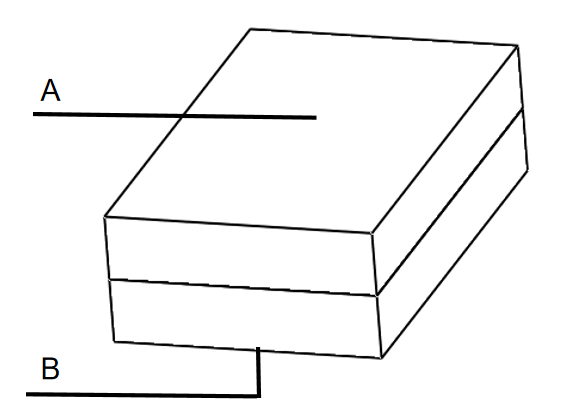
\includegraphics[width=5cm]{figure/双压电晶片示意图.png}
    		\caption{双压电晶片示意图}
    		\label{双压电晶片示意图}
    	\end{minipage}
 
    \begin{minipage}{0.4\textwidth}
    	\centering
    	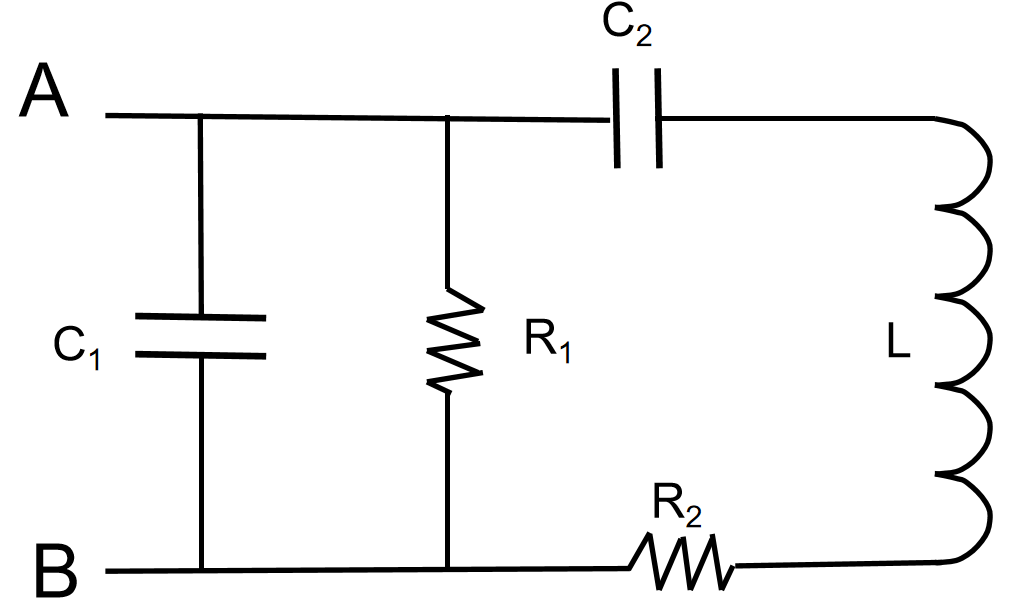
\includegraphics[width=5cm]{figure/双压电晶片等效电路.png}
    	\caption{双压电晶片等效电路图}
    	\label{双压电晶片等效电路图}.
    \end{minipage}
    	
 
    \end{figure}
    双压电晶片如图\ref{双压电晶片示意图}所示,当在AB间施加交流电压时,若片的电场方向与极化方向相同,则下面的方向相反,因此,通过上下一伸一缩,形成超声波振动。双压电晶片的等效电路如图\ref{双压电晶片等效电路图}所示。$C_0$为静电电容,$R$为陶瓷材料介 电损耗并联电阻,$C_m$和$L_m$为陶瓷材料介电损耗并联电阻,$R_m$为损耗串联 电阻。\par
    \newpage
    压电陶瓷晶片有一个固定的谐振频率,即中心频率$f_0$。发射超声波时,加在其上面的交变电压的频率要与它的固有谐振频率一致。这样超声传感器才有较高的灵敏度。当所用的压电材料不变时,改变压电陶瓷晶片的几何尺寸,就可非常方便的改变其固有谐振频率。利用这一特性就可制成各种频率的超声传感器。
    超声波传感器的结构如图\ref{超声换能器结构图}所示,其主要由金属网、外壳、圆锥形振子、双晶振子、底座和引脚等部分组成 。
    \begin{figure}[!h]
    	\centering
    	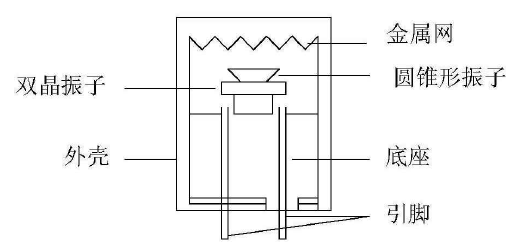
\includegraphics[width=7cm]{figure/超声换能器结构图.png}
    	\caption{超声换能器结构图}
    	\label{超声换能器结构图}
    \end{figure}
\newpage
    \subsubsection{超声波接近传感器的检测原理}
    \begin{figure}[!h]
    	\centering
    	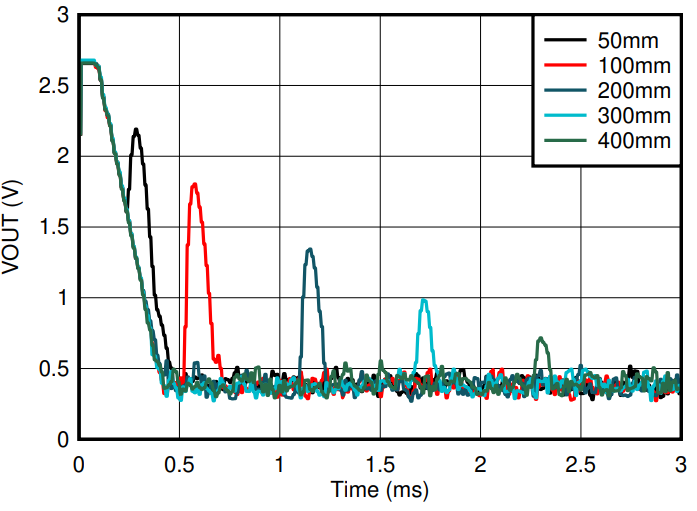
\includegraphics[width=8cm]{figure/VOUT image.png}
    	\caption{VOUT输出}
    	\label{VOUT输出}
    \end{figure}\par
    超声波信号的振幅会随其传播距离的增大而不断减小,通过滤波解调等处理,TUSS4470芯片可将回波信号处理成一个简单的单峰信号,如公式\ref{VOUT公式}以及图\ref{回波接收模块}所示,将不同距离的回波进行处理,可以得到不同峰值的单峰信号,当该峰值信号超过所配置阈值时,芯片OUT4引脚将会发出高电平信号给MCU,MCU以此可以判断物体是否到达指定位置。
    如图\ref{VOUT输出},为20V驱动电压下,不同距离回波进行处理后的输出,可以看到,随着检测距离的增大,输出的峰值在不断减小,也在不断地向右侧进行移动。\par
    在应用中,首先通过SPI接口向芯片寄存器配置输出波形的阈值,当引脚的电压超过所配置的阈值时,即判断为检测到了物体,OUT4引脚拉高,将其作为控制信号连接至MCU。\par
    根据回波解调后的特性,可以知道,当阻碍的物体距离传感器越近时,解调后输出波形波峰的峰值越高,且越靠近左侧,我们可以利用这个特性来调整传感器的最大最小检测距离。如式4.1和式\ref{检测周期公式}所示。
    \begin{align}
    	t&=t_1+t_2+t_3 \\
    	t&_2=\frac{x}{340}
    	\label{检测周期公式}
    \end{align}  
式中\quad$t$---波峰距离起点时间;\par
    \quad$t_1$---脉冲发射时间;\par
    \quad$t_2$---脉冲波在空气中传播时间;\par
    \quad$t_3$---芯片处理回波所花费时间\par         
    当物体距离传感器的距离确定时,其回波信号波峰对应的$t$也是确定的,因此可以通过控制检测窗口来控制检测范围。例如检测范围为$100mm\sim200mm$,其对应的t为$1.2ms\sim2.4ms$,那么我们可以通过程序设计,只对$1.2ms\sim2.4ms$内的OUT4信号进行检测,而屏蔽掉范围外的信号,从而实现只检测$100mm\sim200mm$范围内物体的效果。\par
    TUSS4470驱动芯片还提供了过零检测的功能,通过OUT3引脚输出的过零信号,可对回波频率进行再次检测,增加对其它信号的抗干扰性。该过零信号来自图\ref{TUSS4470芯片功能框图}
    中的对数模块,当信号在其中进行解调时,可根据应用选取特定阶段的信号作为零点。该过零信号仅在OUT4拉高时才有输出,以避免其它噪声的干扰。
    \subsection{超声波接近传感器研究思路与方法}
    本设计的研究思路和方法涉及多个方面。首先,需要明确设计需求,包括测量范围、测量精度、输出格式等要求,以及硬件和软件的设计要求等。接着,根据设计需求,选择合适的硬件平台。本设计选择了CPLD芯片来控制TUSS4470芯片,以实现测距和数据处理等功能。同时,需要选择合适的电源、滤波电路、放大电路等外围电路,以满足系统的实际应用需求。
    
    在硬件平台确定后,需要编写相应的软件程序,实现数据采集、处理、存储和输出等功能。在软件设计过程中,需要考虑到系统的实时性、准确性和稳定性等要求。基于上述硬件和软件设计,搭建系统原型进行实验测试和验证。根据实验结果调整系统设计,优化算法和参数等。
    
    接着,需要对系统进行进一步的集成和优化,包括系统的可靠性、稳定性、抗干扰性等方面的优化。最后,对系统进行全面的测试和验证,包括系统的性能测试、功能测试、可靠性测试等,以确保系统的稳定性和可靠性。
    
    综上所述,制作基于TUSS4470芯片的超声波接近传感器的研究思路和方法需要综合考虑硬件和软件设计的方方面面,并结合实验测试和验证来不断优化和完善系统设计。。